\documentclass[tikz,crop]{standalone}
\usepackage{tikz}
\usepackage{xcolor}
\usepackage{fontspec}
\usepackage{microtype}

%\standaloneenv{tikzpicture}

\setmainfont{C059}
%/usr/share/fonts/gsfonts/C059-Roman.otf

\colorlet{bordercolor}{white} % for final version
%\colorlet{bordercolor}{black} % for debugging

%\definecolor{goldcolor}{cmyk}{0,17,55,50}
\definecolor{goldcolor}{RGB}{132, 117, 78}


\begin{document}
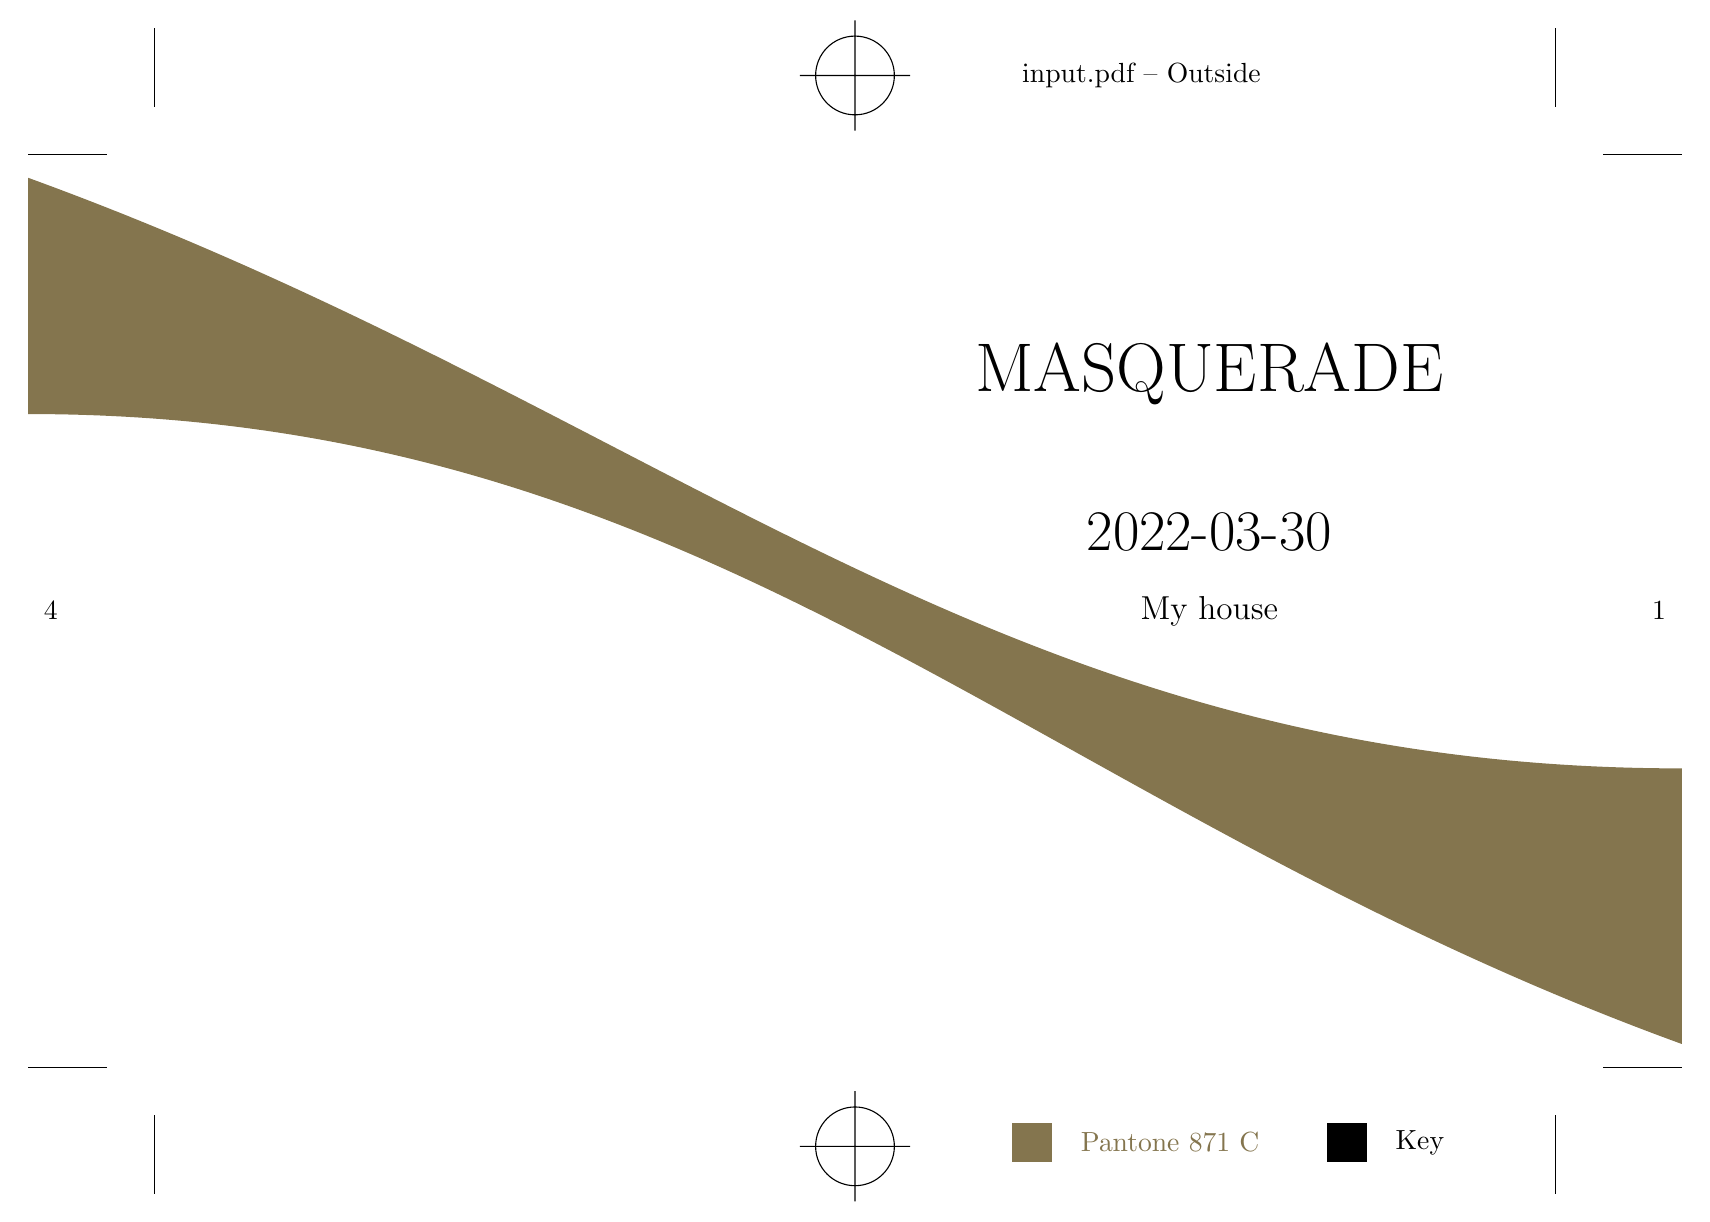
\begin{tikzpicture}[x=1mm, y=1mm]
        \useasboundingbox[draw=bordercolor] (-105, -74) rectangle (105, 74); % A5 paper -> A6 booklet

        % Coca cola sash
        \fill[goldcolor] (-105, 55) to[out=-20,in=180] (105, -20) -- (105, -55) to[out=160, in=0] (-105, 25) -- cycle;

        \node at (45,30) {\Huge MASQUERADE};
        \node at (45,10) {\huge 2022-03-30};
        \node at (45,0) {\large My house};

        % Printer's marks {{{
        \draw (0, 68) circle(5) +(0:-7) -- +(0:7) +(90:-7) -- +(90:7); % Center mark
        \draw (0, -68) circle(5) +(0:-7) -- +(0:7) +(90:-7) -- +(90:7); % Center mark
        \draw  % Crop marks
                (-105, 58) -- (-95, 58) (105, 58) -- (95, 58) %
                (-105, -58) -- (-95, -58) (105, -58) -- (95, -58) %
                (-89, 74) -- (-89, 64) (89, 74) -- (89, 64) %
                (-89, -74) -- (-89, -64) (89, -74) -- (89, -64) %
                ;
        \node[anchor=west, fill=white] at (20,68) {\jobname.pdf -- Outside};
        \node[anchor=west] at (100,0) {1};
        \node[anchor=east] at (-100,0) {4};
        \fill[goldcolor] (20, -65) rectangle +(5, -5) node[midway, right, outer sep=5mm]{Pantone 871 C};
        \fill[black] (60, -65) rectangle +(5, -5) node[midway, right, outer sep=5mm]{Key};
        % }}}
\end{tikzpicture}

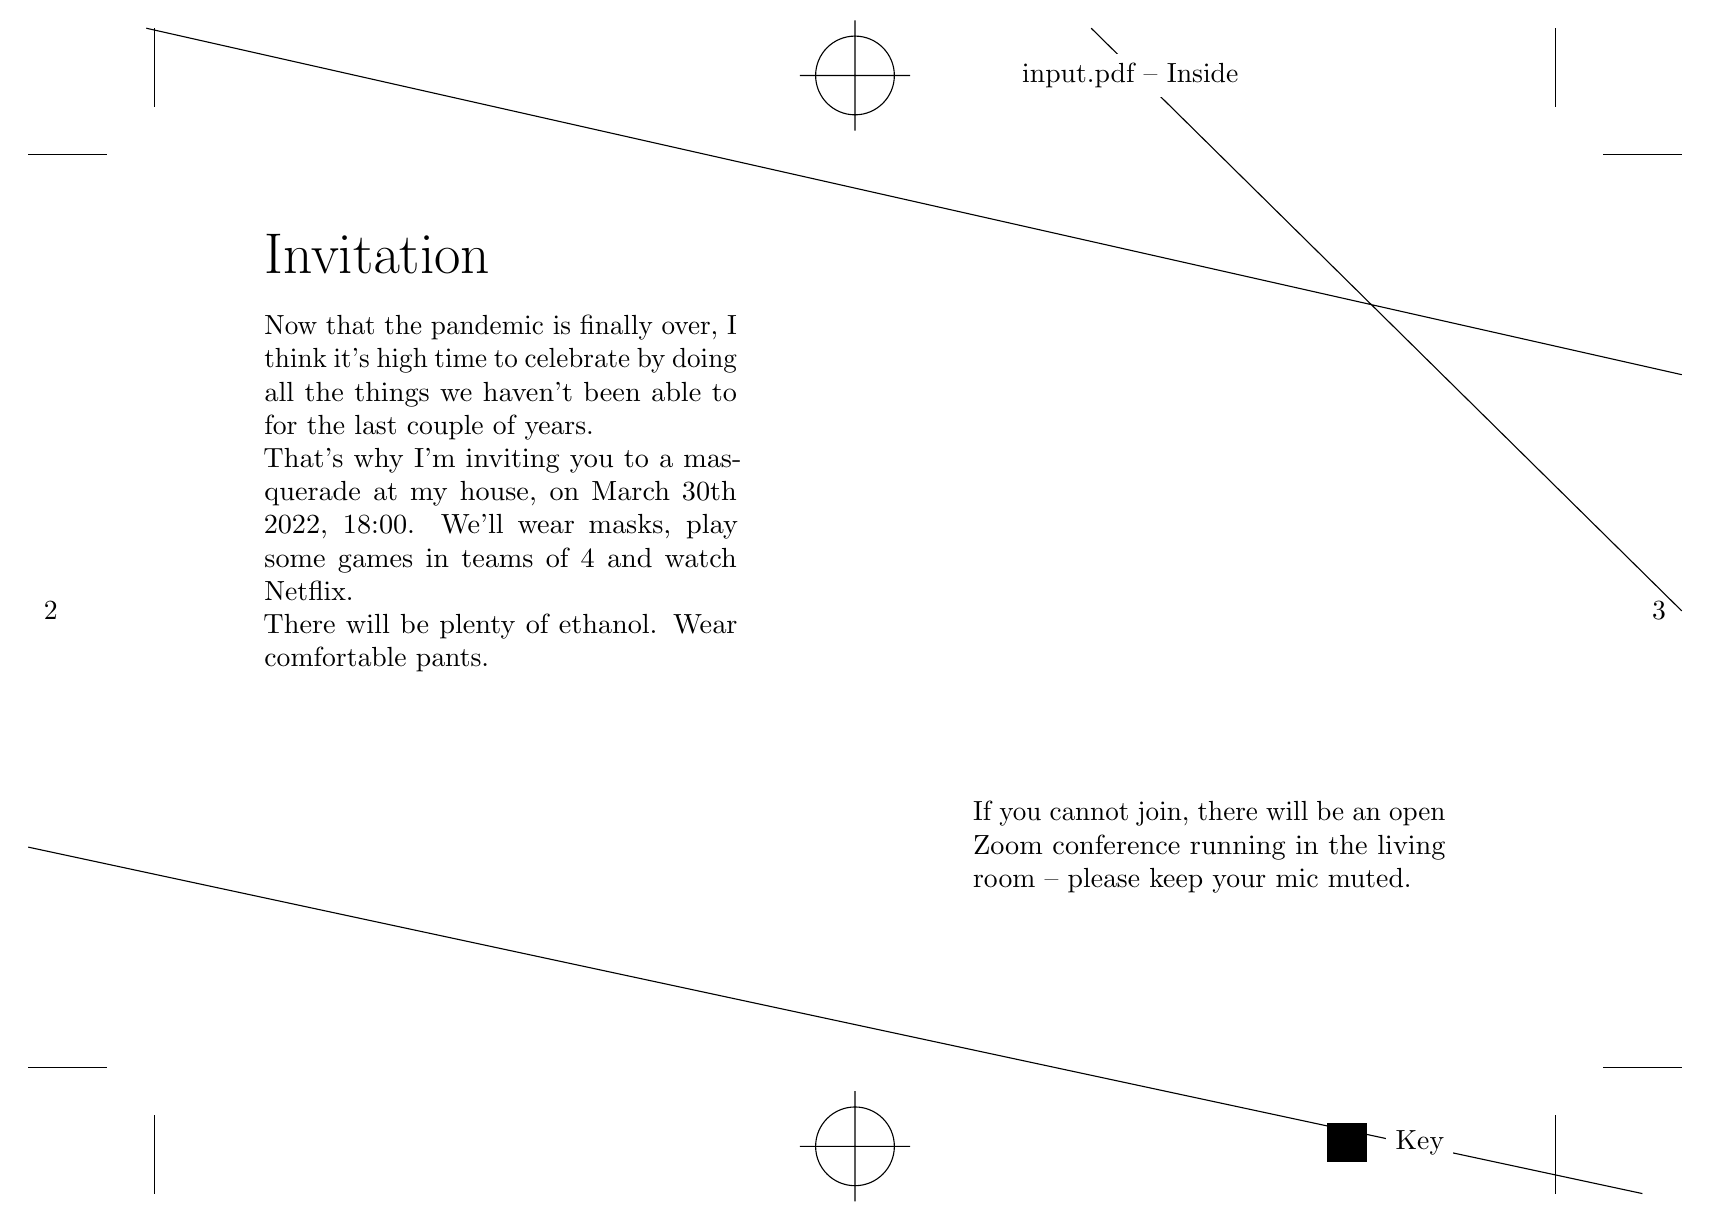
\begin{tikzpicture}[x=1mm, y=1mm]
        \useasboundingbox[draw=bordercolor] (-105, -74) rectangle (105, 74); % A5 paper -> A6 booklet

        \node[text width=60mm,align=justify] at (-45,20){
                        {\huge Invitation}\\[1em]
                        Now that the pandemic is finally over, I think it's
                        high time to celebrate by doing all the things we
                        haven't been able to for the last couple of years.

                        That's why I'm inviting you to a masquerade at my
                        house, on March 30th 2022, 18:00. We'll wear masks,
                        play some games in teams of 4 and watch Netflix.

                        There will be plenty of ethanol. Wear comfortable
                        pants.
                };
        \node[text width=60mm,align=justify] at (45,-30){
                        If you cannot join, there will be an open Zoom
                        conference running in the living room -- please keep
                        your mic muted.
                };

        \draw (30, 74) -- (105, 0) (-90, 74) -- (105,30) (-105, -30) -- (100, -74);

        % Printer's marks {{{
        \draw (0, 68) circle(5) +(0:-7) -- +(0:7) +(90:-7) -- +(90:7); % Center mark
        \draw (0, -68) circle(5) +(0:-7) -- +(0:7) +(90:-7) -- +(90:7); % Center mark
        \draw  % Crop marks
                (-105, 58) -- (-95, 58) (105, 58) -- (95, 58) %
                (-105, -58) -- (-95, -58) (105, -58) -- (95, -58) %
                (-89, 74) -- (-89, 64) (89, 74) -- (89, 64) %
                (-89, -74) -- (-89, -64) (89, -74) -- (89, -64) %
                ;
        \node[anchor=west, fill=white] at (20,68) {\jobname.pdf -- Inside};
        \node[anchor=west] at (100,0) {3};
        \node[anchor=east] at (-100,0) {2};
        %\fill[goldcolor] (20, -65) rectangle +(5, -5) node[midway, right]{\hspace{1em}Pantone 871 C};
        \fill[black] (60, -65) rectangle +(5, -5) node[midway, right, fill=white, outer sep=5mm]{Key};
        % }}}
\end{tikzpicture}

\end{document}
